\documentclass[11pt]{article}
\usepackage[T1]{fontenc}
\usepackage[utf8]{inputenc}
\usepackage{amsmath}
\usepackage{tikz}
\usetikzlibrary{positioning}
\usetikzlibrary{calc}
\usetikzlibrary{fit}

\begin{document}

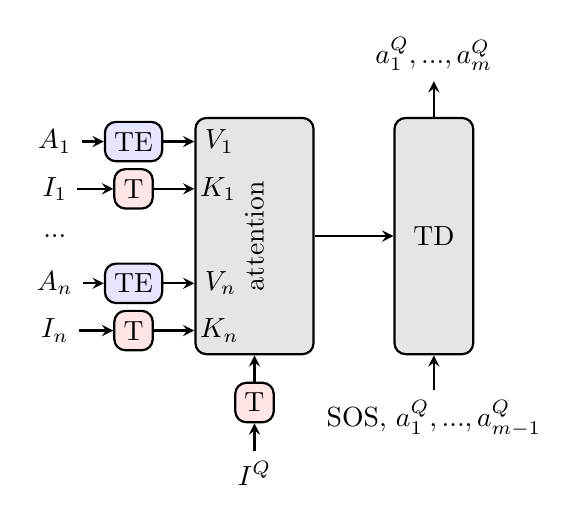
\begin{tikzpicture}[auto, thick, node distance=6mm]
\draw
node at (0, 0) (A1) {$A_1$}
node [below of=A1] (I1) {$I_1$}
node [below of=I1] (dots1) {$...$}
node [below of=dots1] (An) {$A_n$}
node [below of=An] (In) {$I_n$}

node [draw, rectangle, fill=blue!10,rounded corners, right of=A1, minimum height=5mm, node distance=10mm] (At1) {TE}
node [draw, rectangle, fill=red!10,rounded corners, right of=I1, minimum height=5mm, node distance=10mm] (It1) {T}
node [draw, rectangle, fill=blue!10,rounded corners, right of=An, minimum height=5mm, node distance=10mm] (Atn) {TE}
node [draw, rectangle, fill=red!10,rounded corners, right of=In, minimum height=5mm, node distance=10mm] (Itn) {T}

node [draw, rectangle, fill=black!10,rounded corners, right of=dots1, minimum height=15mm, minimum width=30mm, anchor=south, node distance=33mm, rotate=90] (att) {attention}

node at ($(att.west) - (0, 6mm)$) [draw, rectangle, fill=red!10,rounded corners, minimum height=5mm] (Itq) {T}

node [below of=Itq, node distance=9mm] (Iq) {$I^Q$}

node at ($(att.south) + (10mm, 0mm)$) [draw, rectangle, fill=black!10,rounded corners, minimum height=30mm, minimum width=10mm, anchor=west] (TD) {TD}

node at ($(TD.north) + (0, 8mm)$) (outputs) {$a^Q_1, ..., a^Q_{m}$}

node at ($(TD.south) - (0, 8mm)$) (inputs) {SOS, $a^Q_1, ..., a^Q_{m-1}$}
;

\draw[->,>=stealth](A1) -- (At1);
\draw[->,>=stealth](I1) -- (It1);
\draw[->,>=stealth](An) -- (Atn);
\draw[->,>=stealth](In) -- (Itn);

\draw[->,>=stealth](At1) -- node[right,xshift=2mm] {$V_1$}(At1-|att.north);
\draw[->,>=stealth](It1) -- node[right,xshift=2mm] {$K_1$}(It1-|att.north);
\draw[->,>=stealth](Atn) -- node[right,xshift=2mm] {$V_n$}(Atn-|att.north);
\draw[->,>=stealth](Itn) -- node[right,xshift=2mm] {$K_n$}(Itn-|att.north);

\draw[->,>=stealth](Iq) -- (Itq);
\draw[->,>=stealth](Itq) -- (att);

\draw[->,>=stealth](inputs) -- (TD);
\draw[->,>=stealth](TD) -- (outputs);

\draw[->,>=stealth](att.south) -- (TD);

\end{tikzpicture}

\end{document}